% Contesto applicativo

% Stato dell'arte

% Storia e motivi, tutte le volte che il metaverso è stato proposto alla gente e tutte le tecnologie che sono attualmente in uso e anche samsung con il suo vr set del cellulare

\section{Il Metaverso}

    Il concetto di Metaverso nasce nella letteratura di fantascienza, infatti il termine fu coniato da Neal Stephenson nel suo libro \textit{Snow Crash} del 1992. 
    %
    Il termine descriveva uno spazio tridimensionale dove la realtà si univa con un mondo virtuale costantemente attivo.
    %
    Nonostante questo concetto non sia recente, saper dare una definizione di cosa è il Metaverso genera molte difficoltà, infatti è una tecnologia che per la maggior parte ancora non esiste e sebbene riusciamo a ragionare su esperienze tecnologiche future siamo ancora lontani dal rendere possibile questa esperienza.
    %
    Ancora non possiamo sapere quali caratteristiche saranno più importanti e che tipo di dinamiche guideranno la sua formazione, come negli anni '80 era difficile descrivere cosa sarebbe stato internet nel 2022, allo stesso modo è difficile saper descrivere il Metaverso.
    %
    Ad oggi si può dire che il Metaverso è il nuovo principale obiettivo delle grandi compagnie di tecnologia mondiali, come Facebook - non a caso rinominata \textit{Meta} - e Epic Games - azienda proprietaria del motore grafico Unreal Engine e di Fortine, il videogioco che ad oggi viene considerato la piattaforma più vicina al Metaverso che sia stata fatta.

    Matthew Ball, CEO di Epyllion e scrittore di \textit{The Metaverse and How it Will Revolutionize Everything}, lo definisce in questo modo \cite{Ball2022}: 

    \begin{displayquote}
        \textit{Io definisco il metaverso come un network ampiamente scalabile e interoperabile di mondi virtuali 3D renderizzati in tempo reale che possono essere vissuti, in modo sincrono e persistente, da un numero infinito di user effettivi, ciascuno con un senso di presenza individuale, supportando al contempo continuità di dati quali cronologia, identità, comunicazione, pagamenti, diritti e oggetti.}
    \end{displayquote}

    Secondo Matthew Ball il Metaverso è quindi una combinazione di molte tecnologie diverse che collaborano per costruire un'esperienza continua e persistente.
    %
    È l'unione di mondi virtuali, tecnologie - quali visori per la realtà virtuale, dispositivi indossabili e camere a proiezione 3D - e internet.
    %
    È una nuova era della tecnologia che verrà costruita iteramente e lentamente al di sopra delle tecnologie e dei protocolli esistenti che verranno migliorati o sostituiti in base alle esigenze.
    %
    Un ruolo fondamentale lo avranno le piattaforme virtuali, esse infatti daranno effettivamente vita ai mondi virtuali in cui le persone potranno entrare.
    %
    Alcune hanno scopi puramente di intrattenimento - come Roblox, The Legend of Zelda o Minecraft - altri hanno intenti accademici e professionali - come Osso VR o come i simulatori di volo per l'addestramento di piloti.

    La storia del Metaverso è perciò la storia di tutte le piattaforme online e di tutte le tecnologie che stanno contribuendo a costruire mondi ed esperienze virtuali.

    \subsection{Storia del metaverso}
    Sebbene il termine fu coniato nel 1992, il concetto di Metaverso affonda le radici nella letteratura Cyberpunk.
    %
    Tale letteratura comprende romanzi come \textit{True Names di Vernor Vinge} del 1981, che descrive quello che può essere considerato il primo esempio di cyber-spazio, e \textit{Neuromancer di William Gibson} nel 1985, che invece descrive un cyber-spazio dalle caratteristiche molto simili al Metaverso che intendiamo oggi.

    Il primo dei due libri è particolamente importante perché è citato come fonte di ispirazione per il primo gioco nel Metaverso: Habitat \cite{Habitat1990}.

        \subsubsection{Habitat - la prima implementazione di Cyber-spazio}

        
        Habitat viene definito dai creatori un \textit{ambiente virtuale online multigiocatore} \cite{Habitat1990}, ogni utente utilizzava il proprio Personal Computer come frontend comunicando su un network a commutazione di pacchetto con un sistema back-end centralizzato.
        %
        La prima versione di Habitat era stata sviluppata per il Commodore 64 nel 1985 e non era possibile avere stanze virtuali popolose né grafica 3D a causa delle limitate risorse che il modello offriva.
        %
        Nonostante questo, Habitat rese possibile per la prima volta a persone da tutto il mondo di incontrarsi in uno spazio virtuale.
        %
        Gli utenti avevano una rappresentazione virtuale di se stessi in terza persona, questa rappresentazione venne chiamata avatar, come nel romando \textit{True Names}.
        %
        L'utente, attraverso il proprio avatar, aveva la possibilità di interagire con oggetti, parlare con altri avatar attraverso una chat che appariva a schermo in stile "word baloon" e muoversi nel mondo di Habitat composto da un grande numero di posizioni che venivano chiamate \textit{Regioni}.

        \begin{figure}[!ht]
            \centering
            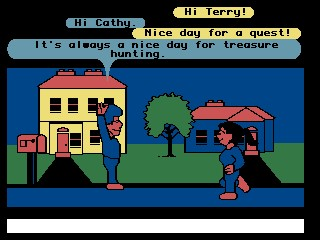
\includegraphics[width=5cm]{figure/lessonshabitat.jpg}
            \caption{Una tipica scena in Habitat.}
        \end{figure}

        Habitat fu un importante progetto che fece capire agli sviluppatori le difficoltà nell'approciarsi alla creazione di un ambiente virtuale multigiocatore e lasciarono in eredità un testo con le lezioni principali che impararono. \cite{Habitat1990}
         
        \subsubsection{Second Life}

        Un altro importante esempio di cyber-spazio è Second Life, una piattaforma online lanciata nel 2003 dalla società Linden Lab.
        %
        Second Life è un ambiente virtuale online multigiocatore 3D e  gli utenti sono rappresentati digitalmente attraverso un avatar tridimensionale.
        %
        Attraverso gli avatar gli utenti hanno la possibilità di socializzare con altri utenti, sia attraverso chat testuale che vocale, esplorare il mondo virtuale, composto da migliaia di regioni chiamate \textit{Sim} e partecipare ad attività di vario genere come concerti, raduni e lezioni e molto altro.
        %
        La particolarità di questa piattaforma, che la distingue da altri videogiochi 3D, è che il contenuto del mondo di gioco viene interamente creato dai giocatori e non c'è un obiettivo da perseguire né una storia.
        %
        Inoltre Second Life possiede una sua economia interna e un token virtuale a circuito chiuso chiamato \textit{Linden Dollar L\$}. 
        %
        Questa valuta non ha valore monetario ma può essere scambiata con Linden Lab per un corrispettivo in dollari.
        %
        Essa può essere usata per comprare, vendere, affittare o commerciale beni e servizi con altri giocatori all'interno del mondo di gioco.
        
        In Second Life per la prima volta brand e organizzazioni parteciparono alla realizzazione di oggetti ed eventi nel mondo virtuale portando il gioco ad evolversi e distaccarsi dall'essere una pura esperienza d'intrattenimento. 
        %
        Brand come Adidas, Calvin Klein e Lacoste lanciarono linee di vestiti indossabili dagli avatar dei giocatori \cite{Fascion2nd} mentre alcune università hanno usato Second Life con obiettivi educativi e formativi, incluse l'Università di Harvard e di Oxford \cite{University2ndLife} ma anche alcune italiane come le università di Milano, di Torino, di Salerno e di altre città. \cite{UnitoIn2ndLife, 2ndLifeWikipedia} 
        %
        Un altro evento importante fu lo sciopero dei lavoratori IBM organizzato su Second Life nel 2007, durante questo sciopero migliaia di avatar contemporaneamente si radunarono per protesta sulla Sim dell'azienda. \cite{2ndLifeWikipedia}
        
        \subsubsection{I visori per la realtà aumentata e virtuale} % qui mettererei i tentativi di samsung

        %Costruzione???
        Un importante contributo alla costruzione del Metaverso lo dobbiamo al avanzamento tecnologico dei dispositivi per la realtà aumentata (AR) e virtuale (VR).
        %
        Questa tecnologia ha accompagnato il concetto del Metaverso sin dai suoi albori.
        %
        %Infatti, troviamo dispositivi simili in \textit{Snow Crash} ma anche nel più recente \textit{Ready Player One}.

        I visori per la realtà aumentata e per la realtà virtuale sono un avanzamento di un dispositivo ottico più antico, lo stereoscopio. 
        %
        Inventato nella prima metà dell'800, lo stereoscopio simula la tridimensionalità del mondo reale per come viene percepita dagli occhi umani. 
        %
        Infatti gli occhi umani trasmettono al cervello due immagini della stessa scena con due punti di osservazione leggermente diversi.
        %
        Il cervello sovrapponendo le due immagini riesce a valutare la distanza degli oggetti: più un oggetto è scostato nelle due immagini più esso viene percepito come vicino, al contrario minore lo scostamento, maggiore è la distanza percepita. \cite{Stereoscopia}

        \begin{figure}[!ht]
            \centering
            %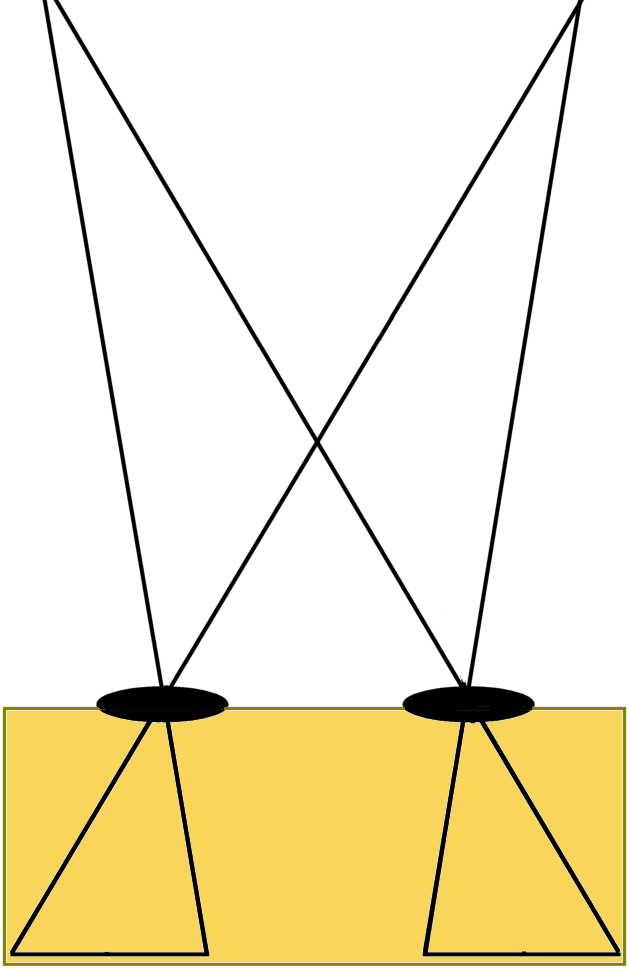
\includegraphics[width=5cm, angle=90]{figure/Stereocamera.png}
            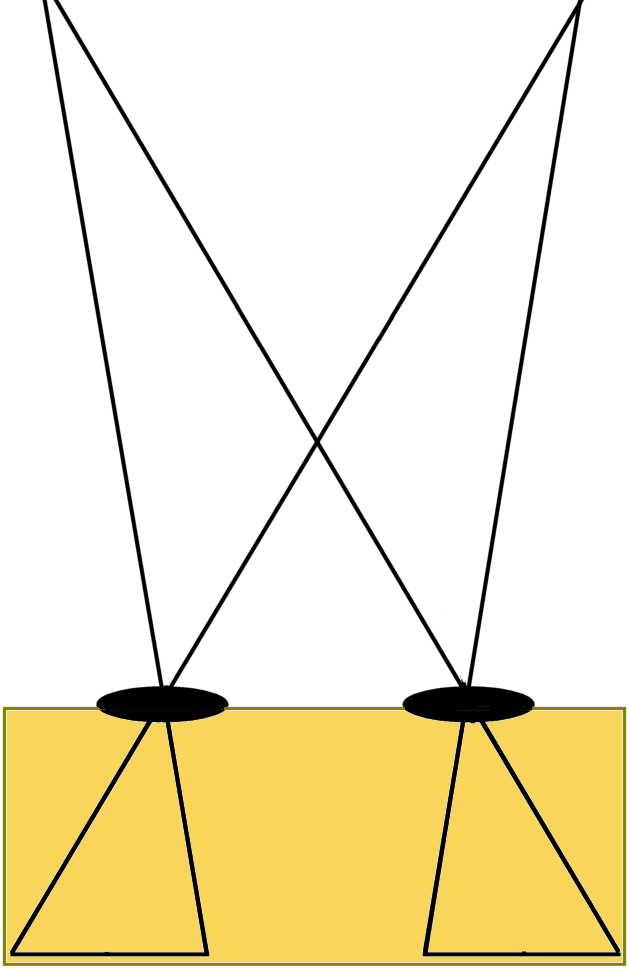
\includegraphics[width=4cm]{figure/Stereocamera.png}
            \caption{Il principio di funzionamento dello stereoscopio.}
        \end{figure}

        Il primo a sfruttare questo principio per immergersi in una realtà simulata fu Ivan Sutherland nel 1968.
        %
        Insieme ai suoi studenti, egli creò il primo sistema di realtà virtuale con visore che permetteva di osservare un ambiente virtuale renderizzato in wire-frame model (metodo che disegna solo gli spigoli di un oggetto 3d).
        %
        Il visore era così pesante che doveva essere appeso al soffito, per questo fu battezzato \textit{La spada di Damocle}.

        Dagli anni '70 fino agli anni '90 i dispositivi AR/VR furono designati quasti esclusivamente per scopi medici, simulazioni di volo, progettazione nell'industria automobilistica e addestramento militare \cite{70and90VR}.
        %
        Bisogna aspettare fino al 1991 per assistere al primo visore VR lanciato sul mercato, ossia quando l'azienda Virtuality Group lanciò la serie 1000 dei prodotti Virtuality che girava sul Commodore Amiga 3000.
        %
        Oltre ai prodotti Virtuality, gli anni '90 videro altre aziende puntare su questa tecnologia, come Sega con l'annuncio del Sega VR e la Nintendo con il lancio del Virtual Boy.

        Dopo allora l'interesse verso i visori da parte di grandi aziende è stato modesto fino al 2010, anno in cui venne prodotto il primo prototipo dell'Oculus Rift.
        %
        Questo visore aveva il tracciamento della posizione, godeva di un angolo di visione di 90° e risolveva i problemi di distorsione che avevano i precedenti visori pre-distorcendo l'immagine renderizzata in tempo reale.
        %
        Inoltre, nel 2013 l'azienda Valve inventò un display a bassa latenza che permise di creare schermi privi di lag e di motion blur indesiderato (il cosiddetto \textit{"smear-effect"}).
        %
        Questo in aggiunta all'avanzamento tecnologico di vari componenti sviluppati per smartphone - giroscopi, sensori di movimento, piccoli schermi HD e processori potenti miniaturizzati - diedero nuova linfa a questa tecnologia e vennero lanciati sul mercato molti modelli di visori.

        
        Nel 2014 Google annunciò Cardboard, una piattaforma per la realtà virtuale fruibile con lo smartphone inserito all'interno di un visore.
        %
        Un simile progetto lo distribuì Samsung nel 2015 con Samsung Gear VR.
        %
        Entrambi i progetti non offrivano un'esperienza coinvolgente e, nonostante fossero economici, non riscossero il successo desiderato e vennero dismessi. 
        %
        Nel 2016 Valve e l'azienda HTC lanciarono l'HTC Vive.
        %
        Questo apparecchio sfruttava una nuova tecnologia chiamata \textit{"room scale"} che permetteva all'utente di muoversi liberamente in una zona di gioco invece di essere vincolato a stare fermo, inoltre i controller erano tracciati grazie a telecamere montate sul visore stesso e grazie ad una serie di sensori che andavano montati nella stanza.
        %
        Sempre nel 2016 l'azienda Sony lanciò il Playstation VR, visore che montava un pannello OLED a 1080p e aveva un angolo di visuale di 100°.
        %
        Questo visore non godeva di componenti di rilievo in confronto ai competitor ma si affacciava ad un mercato diverso, quello delle console. 

        Aggiungere una conclusione

    \subsection{Stato dell'arte}

        \subsubsection{Il progetto Oculus}

        \subsubsection{Il piano di Epig Games}

    \subsection{Prospettive future}

        \subsubsection{Lo sviluppo tecnologico}

\section{Il motore grafico Unreal Engine 5}

\section{Il software di modellazione Blender}

    % focus sul progresso tecnologico che resterà nonostante questa sia una bolla finanziaria che scoppierà

    % Metaverso e blockchain hanno ricevuto tantissimi investimenti anche milionari, e sicuramente questo (anche se il mercato delle crypto fallirà) lascerà dei risultati in termini di avanzamento tecnologico

% Pets.com 

% Tedtalk di Talkman premio nobel economia monete e bitcoin

% The line goes up

% Moonekat canale youtube

% Descrizione pura e asettica senza entrare nel dettaglio economico e senza dire che potrà essere una rivoluzione

% Almeno 80 pagine

% .sol per vedere che cos'è uno smart contract

% cosa esce da un'NFT e cosa si vede

